\chapter{Réalisation et déploiement}

\section*{Introduction}

Ce chapitre décrit la réalisation concrète de l'application
WebCyber : choix technologiques détaillés, construction des images
Docker, configuration de l'instance EC2, mise en place du DNS via
Route\,53, configuration de Nginx avec HTTPS Let's Encrypt, et
procédure de déploiement \textit{from scratch}. Il se termine par le
diagramme de déploiement UML qui synthétise l'ensemble.

\section{Environnement et outils}

\subsection{Poste de développement}

\begin{itemize}
  \item OS : Linux (Ubuntu 24.04);
  \item IDE : Visual Studio Code;
  \item Outils en ligne de commande : \texttt{git}, \texttt{docker},
        \texttt{docker compose}, \texttt{terraform}, \texttt{tfsec},
        \texttt{ssh}, \texttt{curl}, \texttt{dig};
  \item Gestionnaire de versions : Git, dépôt distant sur GitHub.
\end{itemize}

\subsection{Stack technologique retenue}

\begin{table}[H]
\centering
\caption{Synthèse de la pile technologique.}
\begin{tabular}{P{3.5cm} P{4cm} P{6.5cm}}
\toprule
\textbf{Couche} & \textbf{Choix} & \textbf{Justification} \\
\midrule
Cloud / IaaS    & AWS EC2          & Standard du marché, \emph{free tier}, riche écosystème. \\
Système         & Ubuntu 24.04 LTS & LTS, large support Docker. \\
IaC             & Terraform 1.12 + provider AWS 5.98 & Provisionnement déclaratif et reproductible de l'infra. \\
Conteneurs      & Docker + Compose & Reproductibilité, isolation. \\
Registre images & GitHub Container Registry (GHCR) & Distribution de l'image applicative. \\
CI/CD           & GitHub Actions   & Pipeline build / scan / déploiement automatisé. \\
Sécurité IaC    & tfsec (Aqua)     & Analyse statique du code Terraform (\textit{SAST} infra). \\
Proxy / TLS     & Nginx 1.25       & Léger, robuste, terminaison TLS éprouvée. \\
Langage         & Python 3.11      & Productivité, écosystème mature. \\
Framework web   & Flask 3          & Léger, transparent, pédagogique. \\
WSGI            & Gunicorn         & WSGI de production, multi-\emph{worker}. \\
ORM             & SQLAlchemy 2     & Empêche par construction l'injection SQL. \\
Auth            & Flask-Login      & Gestion de session simple et bien testée. \\
Formulaires     & Flask-WTF        & Validation \(+\) CSRF intégrée. \\
Hash mot de passe & Werkzeug PBKDF2-SHA256 & Sel automatique, coût configurable. \\
Base de données & PostgreSQL 16    & Robuste, indexation et JSON natifs. \\
TLS / CA        & Let's Encrypt + Certbot & Certificats gratuits et automatiques. \\
Front-end       & Tailwind CSS     & Mise en page rapide et responsive. \\
\bottomrule
\end{tabular}
\end{table}

\section{Implémentation de l'application Flask}

\subsection{Organisation du code}

Le code source de l'application est structuré selon le \emph{pattern}
\textbf{application factory} de Flask, qui sépare la création de
l'application, les \emph{blueprints} (groupes de routes) et les modèles
de données.

\begin{lstlisting}[language=bash, caption={Arborescence de l'application Flask.}]
app/
├── Dockerfile
├── requirements.txt
├── wsgi.py             # point d'entree Gunicorn
├── config.py           # lecture de l'environnement
├── app.py              # create_app(), init des extensions
├── models.py           # User, Note (SQLAlchemy)
├── forms.py            # LoginForm, RegisterForm, NoteForm
├── routes/
│   ├── auth.py         # /login, /register, /logout
│   └── notes.py        # CRUD, archive, corbeille, recherche
├── templates/          # Jinja2 (auto-escape par defaut)
└── static/             # CSS, JS, images
\end{lstlisting}

\subsection{Modèles SQLAlchemy}

\begin{lstlisting}[language=Python, caption={Extrait de \texttt{models.py}.}]
from flask_sqlalchemy import SQLAlchemy
from werkzeug.security import generate_password_hash, check_password_hash
from flask_login import UserMixin

db = SQLAlchemy()

class User(UserMixin, db.Model):
    __tablename__ = "users"
    id            = db.Column(db.Integer, primary_key=True)
    username      = db.Column(db.String(80),  unique=True, nullable=False)
    email         = db.Column(db.String(120), unique=True, nullable=False)
    password_hash = db.Column(db.String(256), nullable=False)
    created_at    = db.Column(db.DateTime, default=db.func.now())
    notes         = db.relationship("Note", backref="owner", lazy=True)

    def set_password(self, password):
        self.password_hash = generate_password_hash(
            password, method="pbkdf2:sha256"
        )

    def check_password(self, password):
        return check_password_hash(self.password_hash, password)


class Note(db.Model):
    __tablename__ = "notes"
    id           = db.Column(db.Integer, primary_key=True)
    title        = db.Column(db.String(200), nullable=False)
    content      = db.Column(db.Text,       nullable=False)
    user_id      = db.Column(db.Integer, db.ForeignKey("users.id"),
                              nullable=False)
    is_archived  = db.Column(db.Boolean, default=False)
    is_trashed   = db.Column(db.Boolean, default=False)
    created_at   = db.Column(db.DateTime, default=db.func.now())
    updated_at   = db.Column(db.DateTime, default=db.func.now(),
                              onupdate=db.func.now())
\end{lstlisting}

\subsection{Authentification et isolation}

\begin{lstlisting}[language=Python, caption={Extrait du \emph{blueprint} \texttt{notes.py} --- isolation par utilisateur.}]
from flask import Blueprint, request, render_template, redirect, url_for
from flask_login import login_required, current_user
from .models import db, Note

notes_bp = Blueprint("notes", __name__, url_prefix="/notes")

@notes_bp.route("/")
@login_required
def list_notes():
    # Filtre systematique par user_id : isolation des donnees
    notes = (Note.query
                 .filter_by(user_id=current_user.id, is_trashed=False)
                 .order_by(Note.updated_at.desc())
                 .all())
    return render_template("notes/list.html", notes=notes)

@notes_bp.route("/<int:note_id>")
@login_required
def view_note(note_id):
    # 404 si la note n'appartient pas a l'utilisateur courant
    note = (Note.query
                .filter_by(id=note_id, user_id=current_user.id)
                .first_or_404())
    return render_template("notes/view.html", note=note)
\end{lstlisting}

Le \texttt{filter\_by(user\_id=current\_user.id)} sur \emph{toutes} les
requêtes garantit qu'un utilisateur ne peut pas accéder aux notes d'un
autre, même en forgeant un identifiant dans l'URL (parade contre
l'\textbf{IDOR}).

\section{Conteneurisation}

\subsection{Dockerfile applicatif}

\begin{lstlisting}[language=bash, caption={\texttt{app/Dockerfile}.}]
FROM python:3.11-slim

# Securite : utilisateur non-root
RUN useradd -m -u 1000 appuser

WORKDIR /app

# Dependances
COPY requirements.txt .
RUN pip install --no-cache-dir -r requirements.txt

# Code applicatif
COPY . .
RUN chown -R appuser:appuser /app

USER appuser

EXPOSE 5000

# WSGI de production
CMD ["gunicorn", "--bind", "0.0.0.0:5000", "--workers", "2", "wsgi:app"]
\end{lstlisting}

Trois bonnes pratiques sont appliquées : (i)~image \emph{slim} pour
réduire la surface d'attaque, (ii)~création d'un utilisateur
\texttt{appuser} non-root, (iii)~Gunicorn comme serveur WSGI au lieu
du serveur de développement de Flask.

\subsection{Fichier docker-compose.yml}

\begin{lstlisting}[language=bash, caption={\texttt{docker-compose.yml} --- vue conceptuelle.}]
version: "3.8"

services:
  nginx:
    image: nginx:1.25-alpine
    depends_on: [app]
    ports:
      - "80:80"
      - "443:443"
    volumes:
      - ./nginx/nginx.conf:/etc/nginx/nginx.conf:ro
      - ./nginx/conf.d/:/etc/nginx/conf.d/:ro
      - certbot-etc:/etc/letsencrypt
      - certbot-var:/var/lib/letsencrypt
      - ./app/static/:/usr/share/nginx/static/:ro
    restart: unless-stopped
    networks: [webcyber-net]

  app:
    build: ./app
    depends_on: [db]
    env_file: .env
    restart: unless-stopped
    networks: [webcyber-net]

  db:
    image: postgres:15-alpine
    env_file: .env
    volumes:
      - db-data:/var/lib/postgresql/data
    restart: unless-stopped
    networks: [webcyber-net]

networks:
  webcyber-net:
    driver: bridge

volumes:
  db-data:
  certbot-etc:
  certbot-var:
\end{lstlisting}

\section{Infrastructure as Code avec Terraform}

\subsection{Motivation}

Plutôt que de provisionner l'infrastructure manuellement via la console
AWS \---\ démarche peu reproductible et sujette à l'erreur humaine \---,
l'infrastructure est décrite \textbf{en code} avec
\textbf{Terraform}~5.98. Cette approche, dite \emph{Infrastructure as
Code (IaC)}, présente plusieurs avantages :

\begin{itemize}
  \item \textbf{Reproductibilité} : la même configuration peut être
        rejouée à l'identique, en local comme en CI/CD;
  \item \textbf{Versionnement} : le code Terraform est versionné dans
        Git aux côtés du code applicatif;
  \item \textbf{Auditabilité} : chaque modification d'infrastructure
        passe par une \emph{pull request} et un plan d'exécution
        (\texttt{terraform plan}) lisible en revue de code;
  \item \textbf{Analyse statique} : des outils comme \texttt{tfsec}
        peuvent inspecter le code et détecter les mauvaises
        configurations \emph{avant} le déploiement (cf.
        chapitre~\ref{chap:tests}).
\end{itemize}

\subsection{Organisation des fichiers}

\begin{lstlisting}[language=bash, caption={Arborescence du module Terraform.}]
terraform/
|-- provider.tf      # bloc terraform + provider AWS
|-- main.tf          # ressources : data AMI, SG, EC2, EIP association
|-- variables.tf     # declarations de variables
|-- dev.tfvars       # valeurs (gitignore)
|-- vockey.pem       # cle SSH d'AWS Academy (gitignore, chmod 400)
\end{lstlisting}

\subsection{Bloc Terraform et provider}

\begin{lstlisting}[language=bash, caption={\texttt{provider.tf}.}]
terraform {
  required_version = ">= 1.12.0"
  required_providers {
    aws = { source = "hashicorp/aws", version = "5.98.0" }
  }
}

provider "aws" {
  region = "us-east-1"
}
\end{lstlisting}

\subsection{Ressources principales}

Le fichier \texttt{main.tf} décrit trois ressources et une
\textit{data source} :

\begin{enumerate}
  \item \texttt{data "aws\_ami" "ubuntu"} : recherche dynamique de la
        dernière AMI Ubuntu 24.04 LTS publiée par Canonical;
  \item \texttt{aws\_security\_group "ssh"} : règles entrantes 22, 80,
        443 ouvertes au monde, sortantes libres;
  \item \texttt{aws\_instance "instance"} : EC2 t3.micro, IMDSv2
        forcé, \textit{provisioner} \texttt{remote-exec} qui installe
        Docker \(+\) Compose au premier \texttt{apply};
  \item \texttt{aws\_eip\_association "instance"} : association de
        l'Elastic IP existante (\texttt{eipalloc-...}) à la nouvelle
        instance, afin que le DNS reste valide.
\end{enumerate}

\begin{lstlisting}[language=bash, caption={Extrait de \texttt{main.tf} (ressource EC2).}]
# tfsec:ignore:aws-ec2-enable-at-rest-encryption (lab academique)
resource "aws_instance" "instance" {
  ami             = data.aws_ami.ubuntu.id
  instance_type   = var.instance_type
  security_groups = [aws_security_group.ssh.name]
  key_name        = var.key_name

  metadata_options {
    http_endpoint = "enabled"
    http_tokens   = "required"   # IMDSv2 obligatoire
  }

  provisioner "remote-exec" {
    inline = [
      "sudo apt-get update",
      "curl -fsSL https://get.docker.com | sudo sh",
      "sudo usermod -aG docker ubuntu",
      "sudo systemctl enable --now docker"
    ]
    connection {
      type        = "ssh"
      user        = "ubuntu"
      private_key = file(var.private_key_path)
      host        = self.public_ip
    }
  }
  tags = { Name = var.instance_name }
}
\end{lstlisting}

\subsection{Cycle de provisionnement}

\begin{lstlisting}[language=bash, caption={Commandes Terraform.}]
cd terraform/
terraform init                              # telechargement du provider
terraform plan  -var-file="dev.tfvars"      # plan d'execution
terraform apply -var-file="dev.tfvars"      # creation des ressources
terraform destroy -var-file="dev.tfvars"    # destruction propre
\end{lstlisting}

À la fin de l'\texttt{apply}, Terraform affiche les sorties (\textit{outputs}) :

\begin{lstlisting}[language=bash, caption={Sorties typiques après \texttt{apply}.}]
Apply complete! Resources: 3 added, 0 changed, 0 destroyed.

Outputs:
  public_dns = "ec2-54-165-116-113.compute-1.amazonaws.com"
  public_ip  = "54.165.116.113"
\end{lstlisting}

L'EIP étant associée à l'instance, l'adresse publique reste stable
malgré les redémarrages, ce qui maintient la cohérence des
enregistrements DNS de Route\,53.

\section{Configuration DNS via Route\,53}

Sur Route\,53, une zone hébergée publique est créée pour
\texttt{webcyber.app} et deux enregistrements de type A sont ajoutés :

\begin{table}[H]
\centering
\caption{Enregistrements DNS de la zone hébergée \texttt{webcyber.app}.}
\begin{tabular}{P{4cm} C{1.5cm} C{3cm} C{1.5cm}}
\toprule
\textbf{Nom} & \textbf{Type} & \textbf{Valeur} & \textbf{TTL} \\
\midrule
\texttt{webcyber.app}      & A & \(<\)Elastic IP\(>\) & 300 \\
\texttt{www.webcyber.app}  & A & \(<\)Elastic IP\(>\) & 300 \\
\bottomrule
\end{tabular}
\end{table}

Le TLD \texttt{.app} étant inscrit sur la liste \emph{HSTS preload},
le navigateur \textbf{refuse toute connexion non-HTTPS} : la mise en
place de Let's Encrypt est donc obligatoire.

\section{Préparation automatique de l'instance}

À la différence d'une approche manuelle (\texttt{ssh}, \texttt{apt
install}, configuration ligne par ligne), la préparation de l'EC2
est entièrement automatisée par deux mécanismes complémentaires :

\begin{enumerate}
  \item Le \emph{provisioner} \texttt{remote-exec} de Terraform installe
        Docker et active son service au moment du \texttt{terraform
        apply} (cf. extrait de \texttt{main.tf} ci-dessus);
  \item Le pipeline CI/CD (section suivante) clone le dépôt, écrit le
        fichier \texttt{.env} à partir d'un \emph{secret} GitHub, et
        démarre la pile Docker Compose.
\end{enumerate}

Le fichier \texttt{.env} est ainsi \textbf{généré sur le serveur} à
partir d'un secret stocké dans GitHub Actions et \textbf{n'est jamais
versionné}; il est exclu par \texttt{.gitignore}.

\section{Configuration Nginx et HTTPS}

\subsection{Configuration Nginx}

Le proxy Nginx est configuré en deux blocs :

\begin{lstlisting}[language=bash, caption={Extrait \texttt{nginx/conf.d/webcyber.conf}.}]
# Bloc 1 : redirection HTTP -> HTTPS
server {
    listen 80;
    server_name webcyber.app www.webcyber.app;

    location /.well-known/acme-challenge/ {
        root /var/www/certbot;
    }

    location / {
        return 301 https://webcyber.app$request_uri;
    }
}

# Bloc 2 : serveur HTTPS
server {
    listen 443 ssl http2;
    server_name webcyber.app www.webcyber.app;

    ssl_certificate     /etc/letsencrypt/live/webcyber.app/fullchain.pem;
    ssl_certificate_key /etc/letsencrypt/live/webcyber.app/privkey.pem;
    ssl_protocols       TLSv1.2 TLSv1.3;
    ssl_ciphers         HIGH:!aNULL:!MD5;

    # Masquage de la version de Nginx
    server_tokens off;

    # En-tetes de securite
    add_header Strict-Transport-Security "max-age=31536000; includeSubDomains" always;
    add_header X-Content-Type-Options    "nosniff" always;
    add_header X-Frame-Options           "SAMEORIGIN" always;
    add_header Referrer-Policy           "strict-origin-when-cross-origin" always;
    add_header Content-Security-Policy   "default-src 'self'; script-src 'self' 'unsafe-inline'; style-src 'self' 'unsafe-inline'; img-src 'self' data:; font-src 'self' data:; object-src 'none'; base-uri 'self'; frame-ancestors 'self'" always;

    # Tout le trafic : proxy vers Flask
    location / {
        proxy_pass         http://app:5000;
        proxy_set_header   Host              $host;
        proxy_set_header   X-Real-IP         $remote_addr;
        proxy_set_header   X-Forwarded-For   $proxy_add_x_forwarded_for;
        proxy_set_header   X-Forwarded-Proto $scheme;
    }
}
\end{lstlisting}

\paragraph{Détail des en-têtes.}

\begin{table}[H]
\centering
\caption{En-têtes de sécurité HTTP appliqués par Nginx.}
\begin{tabular}{P{4.5cm} P{9cm}}
\toprule
\textbf{En-tête} & \textbf{Rôle} \\
\midrule
\texttt{Strict-Transport-Security} & Force le navigateur à utiliser HTTPS pendant un an (HSTS). \\
\texttt{X-Content-Type-Options}    & Empêche le \textit{MIME-sniffing} (\texttt{nosniff}). \\
\texttt{X-Frame-Options}           & Bloque l'inclusion en \texttt{<iframe>} sauf en \emph{same-origin} (anti-\textit{clickjacking}). \\
\texttt{Referrer-Policy}           & Limite la fuite d'URL via le \emph{referer}. \\
\texttt{Content-Security-Policy}   & Restreint les sources de scripts, styles, images, polices, \ldots\ (défense contre XSS). \\
\texttt{server\_tokens off}        & N'affiche pas la version de Nginx dans les en-têtes (réduction de la divulgation d'information). \\
\bottomrule
\end{tabular}
\end{table}

\subsection{Durcissement des cookies de session Flask}

En complément des en-têtes HTTP, la configuration Flask
(\texttt{app/config.py}) durcit les attributs des cookies de session :

\begin{lstlisting}[language=Python, caption={Extrait de \texttt{config.py} --- cookies de session.}]
class Config:
    FLASK_ENV = os.getenv("FLASK_ENV", "development")

    SESSION_COOKIE_SECURE   = FLASK_ENV == "production"  # cookie envoye uniquement en HTTPS
    SESSION_COOKIE_HTTPONLY = True                       # inaccessible au JavaScript
    SESSION_COOKIE_SAMESITE = "Lax"                      # protection CSRF de base
\end{lstlisting}

Ces trois attributs (\texttt{Secure}, \texttt{HttpOnly},
\texttt{SameSite=Lax}) sont effectivement présents dans la réponse
HTTP, ce qui sera vérifié au chapitre \ref{chap:tests}.

\subsection{Obtention du certificat Let's Encrypt}

L'obtention du certificat suit la méthode \emph{webroot} :

\begin{lstlisting}[language=bash, caption={Première émission du certificat via Certbot.}]
docker run --rm \
  -v certbot-etc:/etc/letsencrypt \
  -v certbot-var:/var/lib/letsencrypt \
  -v ./certbot-webroot:/var/www/certbot \
  certbot/certbot certonly \
  --webroot -w /var/www/certbot \
  -d webcyber.app -d www.webcyber.app \
  --email contact@webcyber.app \
  --agree-tos --no-eff-email
\end{lstlisting}

Une tâche \texttt{cron} quotidienne est ensuite ajoutée pour le
renouvellement automatique :

\begin{lstlisting}[language=bash, caption={Renouvellement automatique des certificats.}]
0 3 * * * cd /home/ubuntu/webcyber && \
  docker run --rm \
    -v certbot-etc:/etc/letsencrypt \
    -v certbot-var:/var/lib/letsencrypt \
    -v ./certbot-webroot:/var/www/certbot \
    certbot/certbot renew --quiet && \
  docker compose exec nginx nginx -s reload
\end{lstlisting}

\subsection{Démarrage de la pile}

En production, la pile est démarrée par le pipeline CI/CD (section
suivante). En local, les commandes suivantes suffisent :

\begin{lstlisting}[language=bash, caption={Démarrage et vérification.}]
docker compose up --build -d
docker compose ps
docker compose logs -f
\end{lstlisting}

\section{Pipeline CI/CD avec GitHub Actions}
\label{sec:cicd}

\subsection{Vue d'ensemble}

L'intégration et le déploiement continus sont assurés par
\textbf{GitHub Actions}. À chaque \emph{push} sur la branche
\texttt{main}, un \emph{workflow} en trois \emph{jobs} séquentiels est
déclenché :

\begin{enumerate}
  \item \textbf{infra-scan} : analyse statique du code Terraform avec
        \texttt{tfsec}; un échec bloque la suite du pipeline;
  \item \textbf{build-and-push} : construction de l'image Docker
        applicative et publication sur le \emph{GitHub Container
        Registry} (GHCR);
  \item \textbf{deploy} : connexion SSH à l'EC2, récupération du
        code, génération du fichier \texttt{.env} depuis un
        \emph{secret}, puis \texttt{docker compose up}.
\end{enumerate}

\begin{table}[H]
\centering
\caption{Étapes du pipeline GitHub Actions.}
\begin{tabular}{C{1cm} P{4cm} P{9cm}}
\toprule
\textbf{\#} & \textbf{Job} & \textbf{Rôle} \\
\midrule
1 & \texttt{infra-scan}      & Scan tfsec sur le dossier \texttt{terraform/} (gate sécurité IaC). \\
2 & \texttt{build-and-push} & \texttt{docker build} + \texttt{push} vers GHCR avec tags \texttt{latest} et \texttt{sha}. \\
3 & \texttt{deploy}         & SSH vers l'EC2, \texttt{docker compose pull \&\& up}, gestion du certificat Let's Encrypt au premier déploiement. \\
\bottomrule
\end{tabular}
\end{table}

\subsection{Extrait du \emph{workflow}}

\begin{lstlisting}[language=bash, caption={\texttt{.github/workflows/deploy.yml} (extrait).}]
name: Build & Deploy
on:
  push:
    branches: [main]

jobs:
  infra-scan:
    name: Terraform Security Scan (tfsec)
    runs-on: ubuntu-latest
    steps:
      - uses: actions/checkout@v4
      - uses: aquasecurity/tfsec-action@v1.0.3
        with:
          working_directory: terraform
          soft_fail: false   # un finding bloque le pipeline

  build-and-push:
    needs: infra-scan
    runs-on: ubuntu-latest
    steps:
      - uses: actions/checkout@v4
      - uses: docker/login-action@v3
        with:
          registry: ghcr.io
          username: ${{ github.actor }}
          password: ${{ secrets.GITHUB_TOKEN }}
      - uses: docker/build-push-action@v5
        with: { context: ., push: true, tags: "ghcr.io/<repo>:latest" }

  deploy:
    needs: build-and-push
    runs-on: ubuntu-latest
    steps:
      - uses: appleboy/ssh-action@v1
        with:
          host:     ${{ secrets.EC2_HOST }}
          username: ${{ secrets.EC2_USER }}
          key:      ${{ secrets.EC2_SSH_KEY }}
          script: |
            git -C "$HOME/webcyber" pull
            printf '%s' "${{ secrets.ENV_FILE }}" > "$HOME/webcyber/.env"
            sudo -E docker compose -f "$HOME/webcyber/docker-compose.yml" pull
            sudo -E docker compose -f "$HOME/webcyber/docker-compose.yml" up -d
\end{lstlisting}

\subsection{Secrets GitHub utilisés}

\begin{table}[H]
\centering
\caption{Secrets configurés dans le dépôt GitHub.}
\begin{tabular}{P{4cm} P{10cm}}
\toprule
\textbf{Nom du secret} & \textbf{Contenu} \\
\midrule
\texttt{EC2\_HOST}    & Adresse IP publique (Elastic IP) de l'instance. \\
\texttt{EC2\_USER}    & \texttt{ubuntu} (utilisateur SSH par défaut). \\
\texttt{EC2\_SSH\_KEY} & Contenu de la clé privée \texttt{vockey.pem}. \\
\texttt{ENV\_FILE}    & Contenu complet du fichier \texttt{.env} (clé secrète Flask, identifiants PostgreSQL, etc.). \\
\bottomrule
\end{tabular}
\end{table}

\subsection{Bénéfices de l'approche}

\begin{itemize}
  \item \textbf{Boucle de retour rapide} : un \emph{push} suffit pour
        livrer l'application en production en quelques minutes.
  \item \textbf{Séparation des responsabilités} : Terraform gère
        l'\emph{infrastructure}, GitHub Actions gère l'\emph{application}.
  \item \textbf{Sécurité par construction} : aucun \texttt{commit}
        contenant une mauvaise configuration Terraform de niveau
        \emph{HIGH} ou \emph{CRITICAL} ne peut atteindre la
        production, grâce au \emph{gate} \texttt{tfsec}.
  \item \textbf{Aucun secret dans le dépôt} : le fichier \texttt{.env}
        et la clé SSH sont stockés exclusivement dans les
        \emph{GitHub Secrets}.
\end{itemize}

\section{Vue d'ensemble du flux HTTPS}

La figure \ref{fig:flux-https} reprend, sous forme synthétique, le
trajet d'une requête HTTPS depuis le navigateur jusqu'à la base de
données, en distinguant clairement la portion \emph{chiffrée} (entre
le client et Nginx) et la portion \emph{en clair sur réseau Docker
isolé} (entre Nginx, Flask et PostgreSQL).

\begin{figure}[H]
  \centering
  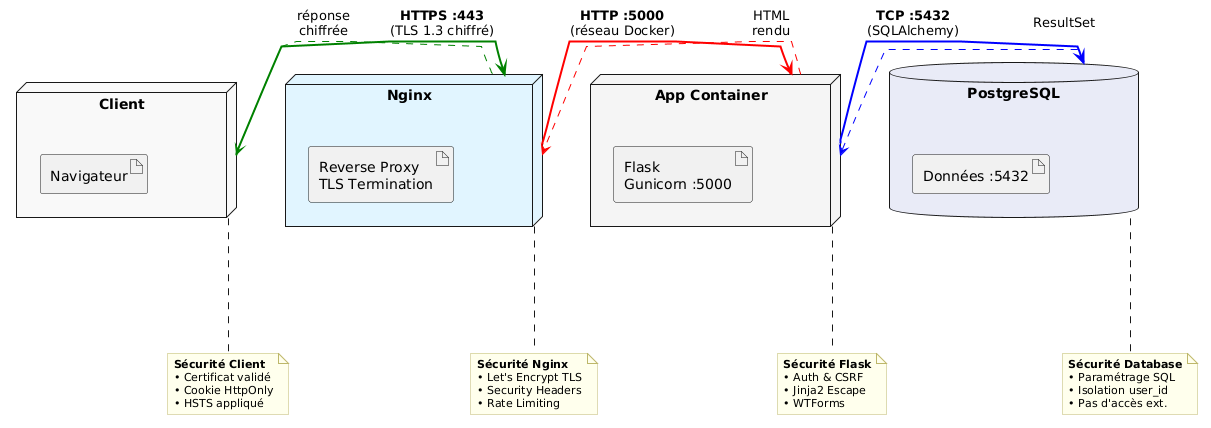
\includegraphics[width=\linewidth]{figures/img/fig08-flux-https.png}
  \caption{Flux d'une requête HTTPS, des en-têtes au stockage.}
  \label{fig:flux-https}
\end{figure}

\subsection{Captures d'écran attendues}

La documentation prévoit l'insertion de captures d'écran illustrant :

\begin{itemize}
  \item l'interface de connexion / inscription ;
  \item le tableau de bord de lecture et de création de notes ;
  \item le résultat du déploiement Docker Compose avec l'état des conteneurs.
\end{itemize}

\begin{figure}[H]
  \centering
  \fbox{\parbox{0.85\linewidth}{\centering
    Capture d'écran 1 : interface de connexion / inscription
  }}
  \caption{Espace réservé pour une capture d'écran du formulaire de connexion.}
  \label{fig:screenshot-login}
\end{figure}

\begin{figure}[H]
  \centering
  \fbox{\parbox{0.85\linewidth}{\centering
    Capture d'écran 2 : interface de gestion des notes
  }}
  \caption{Espace réservé pour une capture d'écran de l'interface de notes.}
  \label{fig:screenshot-notes}
\end{figure}

\section{Diagramme de déploiement}

Le diagramme de déploiement UML (figure \ref{fig:deploiement})
résume les artefacts physiques et logiques mis en jeu, ainsi que les
protocoles de communication entre eux.

\begin{figure}[H]
  \centering
  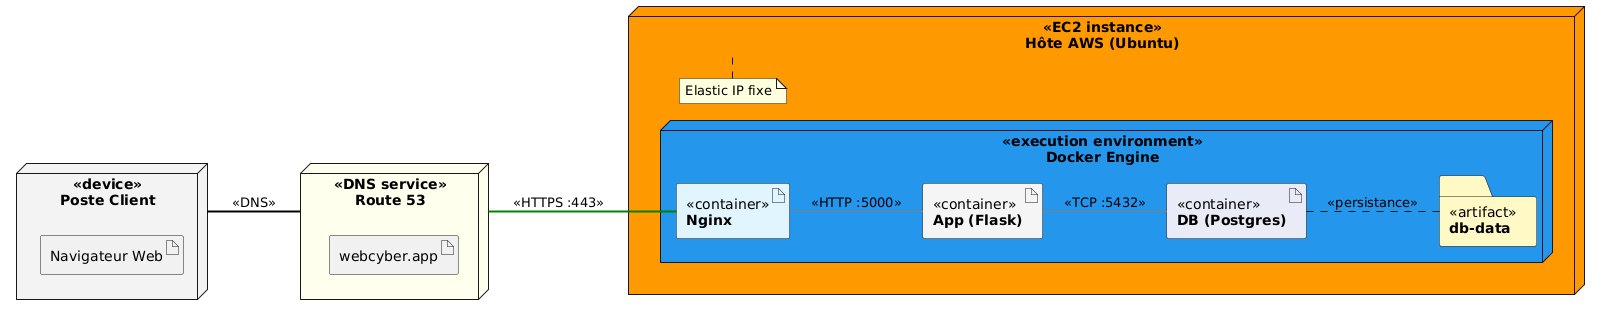
\includegraphics[width=\linewidth]{figures/img/fig10-deploiement.png}
  \caption{Diagramme de déploiement UML.}
  \label{fig:deploiement}
\end{figure}

\section{Conclusion du chapitre}

La réalisation s'est appuyée sur des outils \emph{standards de
l'industrie} (Flask, PostgreSQL, Nginx, Docker, AWS, Let's Encrypt),
ce qui a permis de concentrer l'effort sur l'\textbf{intégration
sécurisée} plutôt que sur la maîtrise de technologies exotiques. Le
résultat : un déploiement reproductible, conteneurisé, accessible en
HTTPS sur \texttt{https://webcyber.app}, et préparé pour la phase de
tests et d'audit qui fait l'objet du chapitre suivant.
